\chapter{Human Centered Design}

\textit{I progettisti devono produrre cose che soddisfino i bisogni della gente, in termini di funzioni, facilità d’uso e gratificazione emotiva. In altre parole, il design (di prodotto) deve essere pensato come un’esperienza totale (per l'utente).} 

[Donald Norman — La caffettiera del masochista]

Le persone sono sempre più frustate dalla complessità degli oggetti quotidiani. Dalla complessità sempre maggiore del cruscotto dell'auto, dalla lavatrice piena di incomprensibili funzioni e pulsanti, dalla crescente automazione della casa, e dalla continua proliferazione di funzioni che i progettisti aggiungono con orgoglio ad ogni nuova versione dei loro prodotti.

La vita della maggior parte degli utenti è ormai diventata una battaglia quotidiana per la sopravvivenza alla invadente e iper-funzionale tecnologia. %tutti i giorni sembra a volte una battaglia infinita contro la confusione, gli errori continui, la frustrazione e un ciclo interminabile di aggiornamenti e manutenzioni degli apparecchi.

Questo problema origina direttamente dalla modalità con la quale vengono oggigiorno progettati gli oggetti quotidiani ed in particolare quelli tecnologici. Le macchine (computer) hanno una modalità di funzionamento logica, dovuta all'algoritmo che il progettista ha sviluppato come anima della macchina. Noi umani invece siamo tutt'altro che logici e razionali, siamo intuitivi, flessibili, versatili e curiosi. È chiaro quindi che nell'interazione uomo-macchina si va a creare una relazione fra specie diverse che hanno modalità di pensiero e di funzionamento opposte.

Gli ingegneri e gli informatici, orgogliosi dei loro progressi tecnologici, hanno preteso da sempre che gli umani si adattassero alle loro macchine. Le macchine sono viste come un elemento di orgoglio che rappresenta il progresso e chi non è in grado di capirle è retrogrado, vecchio e a volte anche un po' stupido.

Questo approccio tecno-centrico dei progettisti ha in realtà leso lo sviluppo stesso della tecnologia dal momento che ne ha rallentato la sua diffusione e accettazione.
La maggior parte degli utenti oggi è frustrata dall'utilizzo di incomprensibili oggetti tecnologici di cui non capisce il principio di funzionamento e dove tipicamente si limita ad utilizzare il 10\% delle funzionalità disponibili.

Le macchine hanno delle loro regole di funzionamento che sono spesso note solo ai progettisti. Quando non si seguono queste regole le cose non vanno come previsto e l'utente si sente stupido ed incapace. La macchina è perfetta, non può sbagliare, quindi se le cose sono andate male è sicuramente colpa dell'umano. 
È vero ma non è l'umano utente ad aver sbagliato, la colpa è del progettista!

Nel design antropocentrico si inverte il paradigma di progettazione mettendo l'utente al centro del processo. Le funzionalità del prodotto vengono dopo. Prima ci sono i bisogni dell'utente!

Questo processo, apparentemente ovvio e banale, risulta in realtà estremamente difficile da applicare per gli informatici. I tecnici infatti amano le funzioni e funzionalità, amano le peculiarità tecniche dei sistemi e sono spesso spinti a sviluppare nuove soluzioni non tanto per risolvere problema ma piuttosto per soddisfazione personale di aver implementato qualcosa che prima non esisteva.

La blockchain è sicuramente un esempio di questo fenomeno. Creata per diletto da degli appassionati di crittografia, ha dato vita alla prima cryptomoneta della storia. Dopo il boom di Bitcoin e delle altre cryptomonete è scoppiata la bolla blockchain dove tutti nel mondo IT hanno iniziato a dichiarare che grazie alla blockchain si sarebbe potuto innovare in maniera radicale tantissimi settori. Ad oggi in realtà dopo aver lanciato numerosi bandi di concorso in tutto il mondo, aver aperto fondi di investimento dedicati alle startup che utilizzano tecnologia blockchain non si è ancora trovata una applicazione di successo, oltre alle cryptomonete, che senza blockchain non sarebbe realizzabile.

Per dirla in altre parole, nessun utente ci ha chiesto di sviluppare la blockchain in quanto tale, c'era bisogno di scambiarsi denaro in maniera alternativa e quindi sono nate le cryptomonete. Ora la corsa a cercare di applicare la blockchain ad altri settori non sta funzionando perché non esiste il problema da risolvere! Stiamo cercando un problema per una tecnologia ma bisognerebbe cercare tecnologie che risolvono problemi!

La morale di questo ragionamento è: se vogliamo progettare tecnologia per le persone dobbiamo capire sia la tecnologia che le persone. Dobbiamo pensare a risolvere i problemi delle persone, non a crearne di nuovi perché dobbiamo bulimicamente sviluppare nuova tecnologia.


Questo vuol dire passare da un approccio tecno-centrico ad uno antropocentrico. Lo human centered desing o HCD, è una \textbf{metodologia di progettazione che parte dai bisogni, dalle capacità e dai comportamenti umani, adattando la progettazione a quei bisogni, quelle capacità e quei comportamenti}. Lo HCD è un approccio di design specificamente orientato allo sviluppo di sistemi interattivi, con l'obiettivo quindi di produrre sistemi utili, altamente usabili e che si \textbf{focalizzino sull'utente}.

Il design antropocentrico è orientato all'efficienza ed all'efficacia e punta quindi ad aumentare la soddisfazione dell'utente durante l'utilizzo del prodotto e ad evitare il più possibile gli effetti negativi e quindi indurre frustrazione.\\

\textbf{Prima l'utente, poi le features!} \\

Lo HCD mette i bisogni, comportamenti e capacità umane prima di tutto e progetta in funzione di esse. Per questo motivo il processo HCD parte dall'osservazione dell'utente, dei suoi comportamenti e quindi dallo studio dei suoi bisogni per poi arrivare solo dopo all'identificazione della tecnologia necessaria.

Il problema principale delle UI è la comunicazione fra uomo e macchina. L'interazione uomo-macchina è una forma di dialogo inter-specie; due soggetti aventi culture, corpi e lingue diverse si trovano a dover interagire per risolvere insieme un problema che uno dei due (l'umano) ha. 
%, in particolare la comunicazione dalla macchina verso l'uomo, \textbf{una buona interfaccia \textit{sa} comunicare con l'utente}.

\begin{figure}[!h]
	\centering
	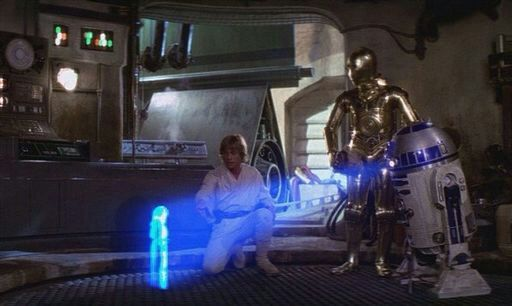
\includegraphics[width=\textwidth]{immagini/starwars.jpg}
	\caption{La tecnologia è percepita come utile quando è possibile comunicarci per risolvere insieme problemi.}
\end{figure}

Progettare interfacce che funzionano fintanto che le cose vanno bene è relativamente facile, ma \textbf{la comunicazione è ancora più importante quando le cose non vanno bene}. È qui che i progettisti devono concentrare l'attenzione, sui casi in cui le cose vanno storte, non su quelli in cui le cose funzionano secondo i piani. 


Dobbiamo smettere di progettare per le persone come vorremmo che fossero e iniziare a progettare per come realmente sono!

Questo approccio è valido sempre, non solo nello sviluppo tecnologico. Un buon avvocato scrive un contratto in previsione di cosa potrebbe andare male nella relazione fra le parti. Se le cose dovessero andare bene sicuramente le parti non avranno bisogno del contratto e questo verrà dimenticato in un cassetto. Il contratto diventa utile quando qualcosa va storto e se ben fatto rende la gestione del problema molto più semplice, veloce e quindi potenzialmente indolore. 

È quindi bene focalizzare sempre l'attenzione su ciò che potrebbe andare storto durante l'interazione così da progettare accuratamente la comunicazione e guidare quindi l'utente verso la risoluzione del problema così da ridurre la frustrazione e quindi la negatività verso il prodotto. 

Non bisogna aver paura che l'utente abbia problemi o che il nostro software abbia degli errori o bug, è inevitabile che questo accada. È importante progettare perché l'utente venga guidato nella risoluzione e gestione dell'errore senza provare frustrazione. Avremo così un utente soddisfatto. 

L'esperienza di utilizzo produce emozioni negli utenti, più emozioni positive (successi) l'utente avrà e migliore sarà la percezione che avrà del nostro prodotto. È importante sottolineare inoltre che la memoria ha la capacità di far provare sensazioni più profonde rispetto al presente. Un utente che di fronte ad un problema riesce a risolverlo perché ben guidato dalla tecnologia avrà memoria di un suo successo. Questo tipo di sensazioni sono molto forti e se associate al prodotto fanno si che l'utente sviluppi empatia per il prodotto e che quindi lo apprezzi e ne senta il bisogno.

L'obiettivo dello HCD deve essere quindi quello di \textbf{creare nell'utente empatia verso il sistema}.

%\textbf{Evitare quindi la frustrazione e aiutare nella risoluzione quando insorge un problema sono i concetti chiave dello HCD.}
%Lo HCD è una filosofia di design che parte dalla \textbf{comprensione delle persone e dei bisogni che esse intendono soddisfare}. Questa comprensione deriva dall'osservazione e dallo studio delle persone che spesso sono inconsapevoli dei loro veri bisogni e magari anche delle difficoltà che incontreranno.

L'HCD è una forma di pensiero ed è quindi compatibile con le varie discipline del design di prodotto che abbiamo precedentemente introdotto (vedere figura \ref{hcd}). 
Si può infatti applicare il pensiero HCD sia al design industriale che alla progettazione dell'interazione o dell'esperienza utente: lo \textbf{HCD non è un'area o un metodo, è una forma di pensiero.}

\begin{table}[!h]
	\center
	\begin{tabular}{ll}
		\multicolumn{2}{c}{\textbf{Il ruolo dello HCD nel design}} \\ \hline
		\multicolumn{1}{c|}{Experience design} & Area di focus     \\ \hline
		\multicolumn{1}{c|}{Industrial design} & Area di focus     \\ \hline
		\multicolumn{1}{c|}{Interaction design} & Area di focus    \\ \hline
		\multicolumn{1}{c|}{Human Centered Design} & \begin{tabular}[c]{@{}l@{}}Il processo che assicura\\ che la progettazione in-\\ contri i bisogni e le ca-\\ pacità degli utenti che \\ useranno il sistema\end{tabular}
	\end{tabular}
\end{table}

%\begin{figure}[!h]
%	\centering
%	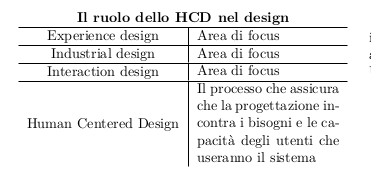
\includegraphics[width=0.7\textwidth]{immagini/HCD}
%	
%	\label{hcd}
%\end{figure}

A sottolineare quanto l'HCD sia ritenuto oggigiorno fondamentale per la progettazione di sistemi destinati all'utilizzo umano, è importante ricordare che il design antropocentrico è ormai parte della norma ISO EU. \\

\textbf{ISO 9241-210:2019 Ergonomics of human-system interaction\\ Part 210: Human-centred design for interactive systems}\\

\textit{This document provides requirements and recommendations for human-centred design principles and activities throughout the life cycle of computer-based interactive systems. It is intended to be used by those managing design processes, and is concerned with ways in which both hardware and software components of interactive systems can enhance human-system interaction.}

\textit{Computer-based interactive systems vary in scale and complexity. Examples include off-the-shelf (shrink-wrap) software products, custom office systems, process control systems, automated banking systems, Web sites and applications, and consumer products such as vending machines, mobile phones and digital television. Throughout this document, such systems are generally referred to as products, systems or services although, for simplicity, sometimes only one term is used. This document provides an overview of human-centred design activities. It does not provide detailed coverage of the methods and techniques required for human-centred design, nor does it address health or safety aspects in detail. Although it addresses the planning and management of human-centred design, it does not address all aspects of project management. }

\textit{The information in this document is intended for use by those responsible for planning and managing projects that design and develop interactive systems. It therefore addresses technical human factors and ergonomics issues only to the extent necessary to allow such individuals to understand their relevance and importance in the design process as a whole. It also provides a framework for human factors and usability professionals involved in human-centred design.}

\textit{Detailed human factors/ergonomics, usability and accessibility issues are dealt with more fully in a number of standards including other parts of ISO 9241 (see Annex A) and ISO 6385, which sets out the broad principles of ergonomics.}

\url{https://www.iso.org/standard/77520.html}\\

Un buon processo HCD parte, come abbiamo detto, dall'osservazione dell'utente e dei suoi bisogni. Tuttavia, tale osservazione non è sempre possibile o facile da attuare. Nei successivi capitoli analizzeremo varie tecniche di prototipazione rapida e metodi di lavoro finalizzati all'estrazione veloce di bisogni utente e all'esecuzione rapida e a basso costo di test. 

Possiamo schematizzare un processo di HCD come un flusso continuo ed iterativo che attraversa le seguenti fasi: 
\begin{itemize}
    \item \textbf{Specificare il contesto d'uso:} identificare gli utenti che utilizzeranno il prodotto, per cosa lo utilizzeranno e sotto quale condizioni e vincoli;
    \item \textbf{Specificare i Requirements:} Identificare i business requirement e gli obiettivi utente che devono essere raggiunti grazie all'utilizzo del software;
    \item \textbf{Progettare la soluzione:} questa fase può essere a sua volta spacchettata in sotto fasi iterative. Si passa tipicamente dadelle bozze a dei prototipi e poi alla soluzione;
    \item \textbf{Testare e valutare:} è fondamentale testare e quindi valutare il sistema così da poter iniziare il ciclo sulla base dei risultati dei test e quindi procedere ad uno sviluppo e miglioramento incrementale.
\end{itemize}

\begin{figure}[!h]
	\centering
	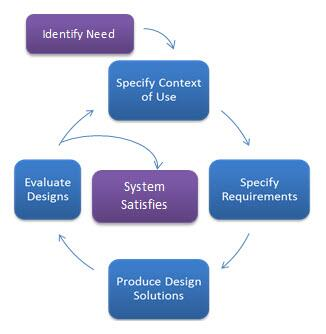
\includegraphics[width=0.8\textwidth]{immagini/HCD-chart}
	\caption{Flusso di lavoro tipico di un processo di design antropocentrico. Fonte: https://www.usability.gov/what-and-why/user-centered-design.html}
	\label{hcd-chart}
\end{figure}

Per ora, al fine di inquadrare meglio la filosofia HCD nel contesto dello sviluppo software vi basti pensare che le versioni alfa e beta dei nostri software possono diventare potenti strumenti di analisi degli utenti. Le versioni di test non servono quindi solamente a fare debugging del codice e delle funzioni, ma servono anche e sopratutto a capire che cosa fanno e come si comportano gli utenti durante l'utilizzo del nostro software.

Nello sviluppo software diventa quindi indispensabile abilitare dei sistemi di tracking dell'utente finalizzati alla produzione di statistiche di utilizzo. Avere zero errori (segnalazioni di bug) su una funzionalità che nessuno usa non vuol dire che questa sia perfetta ma soprattutto vuol dire che non aveva senso implementarla e quindi non ha senso mantenerla. Viceversa, avere alti utilizzi di una funzionale che era stata pensata come opzionale o accessoria ci deve indurre a pensare che invece gli utenti hanno trovato quel processo più utile e soddisfacente rispetto a quello che in fase di progettazione il designer aveva pensato come ``principale'' e quindi fondamentale.


\section{Usabilità}
%Ottenere \textbf{le specifiche dello HCD} è quindi una delle parti più difficili del design stesso, al punto che il principio è quello \textbf{di evitare di specificare il più al lungo possibile} e procedere con ripetute approssimazioni: si esegue una specifica ad alto livello, se ne implementa una parte, si testa sull'utente finale e tramite il suo feedback, si modifica la parte implementata e la si testa di nuovo. Fatto ciò si passa, magari momentaneamente, ad implementare un'altra parte.

Secondo la norma ISO, per usabilità si intende il \textit{``grado in cui un prodotto può essere usato da particolari utenti per raggiungere certi obiettivi con efficacia, efficienza e soddisfazione in uno specifico contesto d’uso''.} 

Sul sito dell'Agenzia per l'Italia digitale (\url{https://www.agid.gov.it/it/design-servizi/usabilita}) si legge: \\

\textit{L'usabilità è un carattere imprescindibile nella realizzazione di un portale web, perché permette di creare un ambiente familiare per l'utente, determinando numerosi vantaggi:}

\begin{itemize}
    \item \textit{consente di trovare e comprendere informazioni in modo più semplice e intuitivo;}
    \item \textit{facilita la memorizzazione e l'apprendimento dei contenuti presenti;}
    \item \textit{permette una riduzione dei costi e degli errori di sviluppo;}
    \item \textit{rende l'utente più autonomo e sicuro nel rapporto con lo strumento.}
\end{itemize}

\textit{L'usabilità mira a ridurre la distanza tra il cittadino e le amministrazioni, permettendo agli utenti di trovare le informazioni necessarie, comprenderne i contenuti ed eliminare le difficoltà di utilizzo di un determinato sito istituzionale.}\\

Si nota subito che il tema dell'usabilità è spesso associato esclusivamente al mondo del web e dello sviluppo di siti internet. L'usabilità è quindi intesa come la disciplina che regola la costruzione del sito o applicazione sulla base delle esigenze dell’utente, cercando di semplificare la sua esperienza di navigazione.

Questa è ovviamente un'errata semplificazione dovuta a come in diversi settori dell'informatica si siano adottate terminologie diverse per esprimere concetti simili se non equivalenti. Nel mondo del design di oggetti interattivi per esempio, l'usabilità è talmente importante che viene quasi data per assodata e il suo studio è spacchettato in diverse sotto attività e quindi risulta più raro trovare delle attività dedicate allo studio dell'usabilità in quanto tale.

Il tema dell'usabilità e del design antropocentrico si applicano (si dovrebbero applicare) quindi, a tutto il mondo dello sviluppo di prodotto. Ogni oggetto, artefatto, software o sistema destinato all'utilizzo da parte di utenti (umani) necessita che se ne studi la relativa usabilità e che intorno a questa si progetti il sistema stesso (HCD).

Una risorsa molto interessante e ben fatta sul tema dell'usabilità di servizi destinati ai cittadini è \url{https://designers.italia.it/}. Sul portale, nato nel 2017, sono presenti numerose linee guida e forum di conversazione relativi allo sviluppo di software per la Pubblica Amministrazione. 

\begin{figure}[!h]
	\centering
	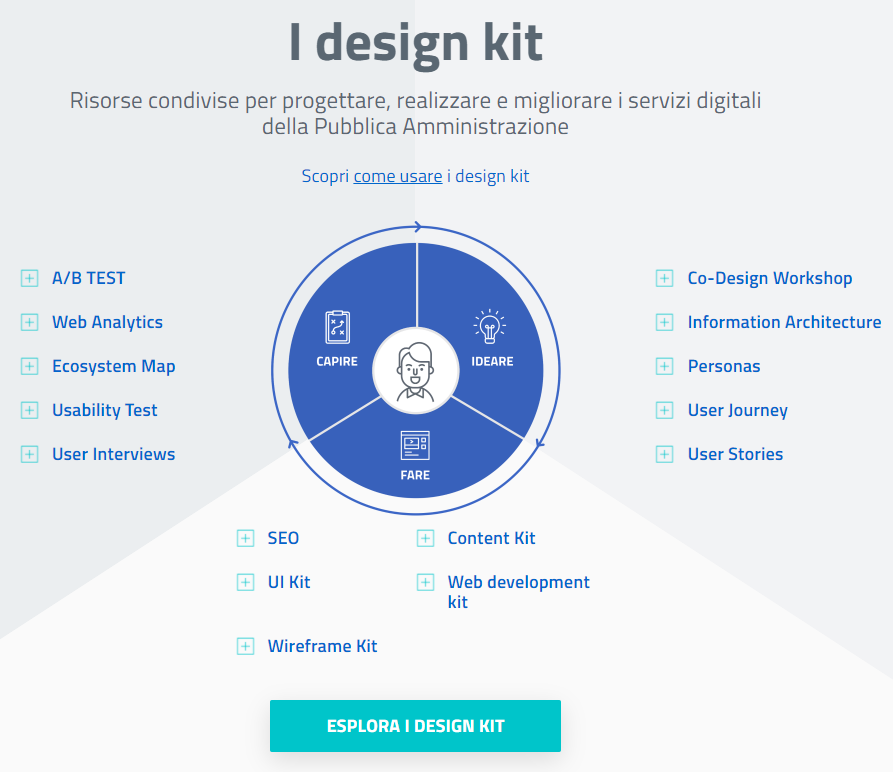
\includegraphics[width=0.8\textwidth]{immagini/designeritalia}
	\caption{https://designers.italia.it/ Mette a disposizione varie linee guida e strumenti per la progettazione antropocentrica di servizi dedicati alla pubblica amministrazione.}
	\label{designersitalia}
\end{figure}
